\leadchapter{
  ABSTRACT
}

\chapter[][]{A numerical exploration of thinned Hawkes processes through spectral theory}\label{chapter:spectral_thinning}

\section{Introduction}

The Hawkes process model introduced for the first time in \textcite{Hawkes1971} is a kind of past-dependant point process used to model self-exciting interactions among event times. 
Its applications are numerous among various fields with examples in sociology \parencite{Linderman2014},
biology \parencite{Gupta2018, Lambert2018, Rizoiu2018},
seismology \parencite{Ogata1988, Ogata1998}
and finance \parencite{Bacry2013, Bacry2015, Hawkes2018}, to mention a few.

As a result, there is many efforts around proposing estimation methods. Traditional methods include maximum likelihood estimators \parencite{Ogata1978, Ozaki1979}, least-square error minimisation \parencite{Reynaud2014,Bacry2020}, method of moments \parencite{DaFonseca2013}, in both parametric and non-parametric contexts.

Most of these methods tend to study the model under the assumption that there is no missing data in the samples used for estimation. 
However, if this assumption does not hold, it is common for estimators to be biaised or even for theoretical properties to not longer be valid.
Some works in the literature consider different missing or imperfect data contexts such as binned observations in \textcite{Cheysson2022}, jittering (or random displacement) as exemplified in \textcite{Antoniadis2006,Bonnet2022}, superposition as in \textcite{Bonnet2024}. 

In particular, jittering and superposition are two of the three most common operations on point processes, along with thinning.
Thinning is more often used in simulation scenarios for point processes, 
with the main example being Ogata's thinning procedure as introduced in \parencite{Ogata1981} or to accelerate estimations as a method of undersampling \parencite{Li2019}.
Nonetheless, the use of thinning to model missing data is scarcer in the literature, 
which could be useful in order to account for sporadic detection errors.

A main work focusing on noised data for both point processes and proposing numerical applications to Hawkes processes can be found in \textcite{Lund2000}. 
Authors propose a conditional log-likelihood model for point process that have been noised through the three classic operations in the field: jittering, superposition and thinning. 
Their method consists on establishing an expression of such a log-likelihood when the base point process (or an estimation of it) is available.
They obtain an approximation of a maximiser through some simplifications and an iterative optimisation on a small space of parameters.
The main obstacle that arises in this context is that it is essential to have some information on the ground process in order to estimate the underlying effects of noise.

In this chapter, we take inspiration from the spectral estimation methods as presented in \textcite{Cheysson2022, Bonnet2024}.
Spectral theory for point processes was properly introduced for the first time in \textcite{Bartlett1963},
focused around the Bartlett spectrum. 
Works concerning the spectral study and estimation of point processes appeared in the literature with numerous theoretical approaches in temporal and spatial contexts \textcite{Daley1971, Tuan1981, Mugglestone2001, Rajala2023}.

In our work, we explicit the form of the Bartlett spectrum for a point process thinned with independent and identically distributed probabilities. In particular, we follow a similar scheme as the one presented for the superposition of point processes in \textcite{Bonnet2024}, with a particular interest in the univariate Hawkes process with exponential kernel.

We illustrate the performance of our estimators for different levels of thinning and show the importance of accounting for eventual missing data in the context of point processes.

Additionnaly, we carry out a numerical study in a different context:
a main issue when working with point observations, specially issued from real data, is the low amount of repetitions and information available.
Common methods to circumvent this problem include considering penalised contrasts for optimisation methods along with subsampling or cross-validation frameworks. 
This is however a complicated issue in point processes, as common methods like splitting data can be difficult for low counts of points, and may wash-out interaction among points (as suggested in \textcite{Reynaud2014}).
An example of the difficulties and uses of cross-validation for point patterns can be found in \textcite{Cronie2023}.
In this chapter, we leverage the thinning operation in order to create \textit{subsamples} of a single Hawkes process
and show that, through a penalised version of the spectral log-likelihood, 
it is possible to improve the obtained estimators.

PRESENTER CHAPITRES UNE FOIS STABILISÉ

\section{Mathematical setting}\label{sec:chap5_mathsetting}

\subsection{The $p$-thinning of point processes}\label{sec:chap5_hawkesprocess}

In this chapter, we will focus our study on the stationary univariate Hawkes process on the real line $\RR$, noted $H$.
The Hawkes process can be characterised by its conditional intensity function, for all $t\in\RR$:
\begin{equation}\label{eq:chap5_hawkes_intensity}
    \lambda(t) = \mu + \int_{-\infty}^{t}{h(t-s)\,H(\dd s)} = \mu + \sum_{T_k \leq t}{h(t-T_k)}\,,
\end{equation}
where $\mu > 0$ is the baseline intensity, and $h\colon\RR\to \RR_{\geq 0}$ is the kernel function modelling the self-exciting behaviour of past points $(T_k)_{k\in\ZZ}$.

In order for $H$ to be a point process (\ie an a.s. finite measure in any bounded set $B$), 
a sufficient and necessary condition \parencite{Hawkes1971} is that 
\[\|h\|_1 = \int_{\RR}{h(t)\,\dd t} < 1\,.\]
Furthermore, let $\mathcal{B}_{\RR}^c$ denote the set of bounded Borel sets on $\RR$, and let, for any $B\in\mathcal{B}_{\RR}^c$:
\[H(B) = \sum_{k\in\ZZ}{\II_{T_k \in B}}\,,\]
be the number of event times in $B$. 

In this chapter, we will study a thinned version of process $H$ defined as follows:
\begin{definition}\label{def:chap5_thinning}
For any $p\in(0,1]$, we denote $H_p$ a $p$-thinning of a point process $H$, defined for any $B\in\mathcal{B}_{\RR}^c$ as:
\[H_p(B) = \sum_{k\in\ZZ}{\II_{T_k \in B} Z_k}\,,\]
where $(Z_k)$ is an i.i.d. collection of Bernoulli random variables of parameter $p$.
\end{definition}

In practice, the event times of process $H_p$ correspond to a subset of $(T_k)_{k\in\ZZ}$ where each point
is erased with a random probability $1-p$. 
Setting $p = 1$ keeps all original points from process $H$ which is not a proper thinning per se,
but we include this value in order to lighten notations in the incoming sections. 

\subsection{Spectral theory for point processes}\label{sec:chap5_spectral_theory}

For a point process $H$, we define the first and second-order measures $M_1, M_2$, for any $A, B\in\mathcal{B}_{\RR}^c$, as:
\[M_1(A) = \EE[H(A)]\,,\qquad M_2(A,B) = \EE[H(A)H(B)]\,.\]
Under stationarity conditions, it follows that \parencite[Proposition 8.1.I]{DaleyV1}, for any $A, B\in\mathcal{B}_{\RR}^c$:
\[M_1(A) = m_1 \ell_{\RR}(A)\,,\]
where $m_1 = \EE[H([0,1])]$ is usually known as the average intensity of process $H$.

The spectral analysis approach of point processes is based on the Bartlett spectrum $\Gamma$ \parencite{Bartlett1963}, 
a measure on $\RR$ associated to the second-order moment measure $M_2$. 
To introduce it properly, let us consider the Schwartz space $\mathcal{S}$ defined as:
\[
    \mathcal S = \left\{ f \in C^\infty, \forall k \in \{1, 2, \dots\}, \forall r \in \{1, 2, \dots\},
    \sup_{x \in \RR} \left| x^r
    f^{(k)}(x)
    \right| < \infty \right\}\,,
\] where $C^\infty$ denotes the set of infinitely differentiable functions $f$ from $\RR$ to $\RR$, 
and $f^{(k)}$ denotes the $k^{th}$-order derivative of $f$.
In particular, for any $f\in\mathcal{S}$, we define its Fourier transform $\tilde f$, for any $\omega\in\RR$, as:
\[\tilde f (\omega) = \int_{\RR}{f(x) \mathrm{e}^{-2\pi\iu x \omega}\,\dd x}\,.\]

The Bartlett spectrum of a point process $H$ is the measure $\Gamma$ such that, 
for any $\varphi\in\mathcal{S}$ \parencite[Definition 2]{Bremaud2005}:
\begin{equation}\label{eq:chap5_bartlett_variance}
    \VV\left[\int_{\RR}{\varphi(x)H(\dd x)}\right] = \int_{\RR}{|\tilde\varphi(\omega)|^2\Gamma(\dd \omega)}\,.
\end{equation}
Existence of such a measure is esablished for any stationary point process \parencite[Proposition 8.2.I.(a)]{DaleyV1},
and by polarisation of Equation~\eqref{eq:chap5_bartlett_variance}, we obtain for any $\varphi, \psi \in \mathcal{S}$:
\begin{equation}\label{eq:chap5_bartlett_covariance}
    \Cov\left(\int_{\RR}{\varphi(x)H(\dd x)}, \int_{\RR}{\psi(x)H(\dd x)}\right) = \int_{\RR}{\tilde \varphi(\omega)\tilde \psi(-\omega)\Gamma(\dd \omega)}\,.
\end{equation}

Whenever $\Gamma$ is an absolutely continous measure, we denote $f:\RR\to \CC$ its Radon-Nikodym derivative, 
known as the spectral density of process $H$.

Another important quantity in the spectral theory of point processes is the periodogram $I^T\colon \RR \to \CC$:
for a realisation $(T_k)_{k=1:N(T)}$ of a process $H$ in a time window $[0,T]$, the periodogram is defined, for all $\omega\in\RR$, as:
\[I^T(\omega) = \frac{1}{T}\sum_{k=1}^{N(T)}\sum_{l=1}^{N(t)}{\mathrm{e}^{-2\pi \iu \omega (T_k - T_l)}}\,.\]

Furthermore, for any sequence $(\omega_k)_{k=1:M}$, such that $\omega_k \neq \omega_l$, for all integers $k\neq l$,
the random variables $(I^T(\omega_k))_{k=1:M}$ are asymptotically independent and exponentially distributed \parencite{Tuan1981} with respective parameter $(1/f(\omega_k))_{k=1:M}$.

In this chapter, we will work on a parametric setting, 
so let us assume that we dispose of a statistical model for the spectral density defined as:
\[
    \mathcal{P} = \left\{
        f_\theta \colon \RR \to \CC \colon \theta \in \Theta
    \right\}\,.
\]
We can then define the \textit{spectral} log-likelihood $\ell_T(\theta)$ for an observation $(T_k)_{k=1:N(T)}$ of $H$ as:
\begin{equation}\label{eq:chap5_spectral_ll}
    \ell_T(\theta) = -\frac{1}{T}\sum_{k=1}^{M}{\log(f_\theta (\omega_k)) + \frac{I^T(\omega_k)}{f_\theta(\omega_k)}}\,.
\end{equation}

We can then introduce the Whittle estimator $\hat \theta$ \parencite{Whittle1952} as:
\[\hat \theta = \arg\max_{\theta \in \Theta}~ \ell_T (\theta)\,.\]

\section{Parametric estimation of a thinned process}\label{sec:chap5_estimation}

\subsection{The spectrum of a thinned point process}

The goal of this chapter is to establish a parametric estimation method for the observation of a thinned Hawkes process.
We will then begin by establishing the expression of a $p$-thinning of a point process. 
We will leverage the study of spectral quantities on marked point process, 
which can be found in \textcite{Bremaud2002, Bremaud2005}. 

For this, let us introduce an alternative way of viewing the $p$-thinning of a point process through marked point process theory.
In this section, $H$ will denote a stationary point process on $\RR$ with spectral density function $f$.

We define the marked point process $\bar H$ associated to $H$, with marks $Z_k$ on a metric space $\mathcal{K}$ as the collection of points
$(T_k, Z_k)_{k\in\ZZ} \in (\RR \times \mathcal{K})^{\ZZ}$ (see \textcite[Chapter 6.4]{DaleyV1} for a more thorough presentation of marked point processes). 
The random marks $Z_k$ are usually used to represent underlying information on the event times of a point process $H$, 
which is often referred to as the \textit{ground} process.
In our work, we will restrict ourselves to the case where the random variables $(Z_k)_{k\in\ZZ}$ are independent and identically distributed.
In this way, process $\bar H$ is well-defined \parencite[6.4.IV(a)]{DaleyV1}.

We can then view a $p$-thinning of $H$ as a marked version $\bar H$ where $\mathcal{K} = [0,1]$
and the $(Z_k)_{k\in\ZZ}$ are a collection of Bernoulli random variables of parameter $p$.
This way we may define the thinned process $H_p$, for any $B\in\mathcal{B}^c$, as:
\[H_p(B) = \bar H(B\times\{1\})\,.\]

Under this scope, we will apply the results of \textcite{Bremaud2005}, 
that we adapt to our notations here as:

\begin{theorem}[{\textcite[Theorem 2]{Bremaud2005}}]\label{th:chap5_spectral_marked}
    Let $H$ be a stationary point process with Bartlett spectrum measure $\Gamma$ and 
    let $\bar H$ be a marked version of $H$ with i.i.d. marks $Z_k$ with shared distribution $Z$ on a metric space $\mathcal{K}$.
    Let $\varphi^\star, \psi^\star$ be measurable functions from $\RR \times \mathcal{K} \to \RR$, 
    such that:
    \begin{itemize}
        \item $\displaystyle
            \int_{\RR}{\EE\left[|\varphi^\star(x, Z)|\right]\dd(x)} < +\infty\,,\qquad \int_{\RR}{\EE\left[|\psi^\star(x, Z)|\right]\dd(x)} < +\infty\,.
        $
        \item $\displaystyle
            \int_{\RR}{\EE\left[\varphi^\star(x, Z)^2\right]\dd(x)} < +\infty\,,\qquad\int_{\RR}{\EE\left[\psi^\star(x, Z)^2\right]\dd(x)} < +\infty\,.
        $
        \item By denoting $\bar \varphi : x\to \EE\left[\varphi^\star(x, Z)\right]$ and $\bar \psi : x\to \EE\left[\psi^\star(x, Z)\right]$, then,
              \[\bar \varphi,\bar \psi \in\mathcal{S}\,.\]
    \end{itemize}

    Then, it follows that:
    \begin{equation}\label{eq:chap5_marked_spectrum}
        \Cov\left(\sum_{k\in\ZZ}{\varphi^\star(T_k, Z_k)}, \sum_{k\in\ZZ}{\psi^\star(T_k, Z_k)}\right) = 
        \int_{\RR}{\tilde {\bar\varphi} (\omega) \tilde{\bar \psi} (-\omega)\,\Gamma(\dd \omega)} 
        + \int_{\RR}{\Cov\left( \tilde \varphi^\star(\omega, Z), \tilde \psi^\star (-\omega, Z)\right)M_1(\dd \omega)}\,,
    \end{equation}
    where, for any $\omega\in\RR$, $\tilde \varphi^\star(\omega, Z)$ (resp. $\tilde \psi^\star(\omega, Z)$) denotes the Fourier transform of the function $x\to \varphi^\star(x, Z)$ (resp. $x\to \psi^\star(x, Z)$).
\end{theorem}

The utility of this result resides on the link that it established between the covariance of a marked point process $\bar H$
and the Bartlett spectrum of its ground process $H$. 
This allows to establish an explicit expression of the spectral density of the $p$-thinning of a process $H$, 
as presented in the following proposition:

\begin{proposition}\label{prop:chap5_spectral_thinning}
    Let $H$ be a stationary point process admitting a Bartlett spectrum $\Gamma^N$ defined as in Equation~\eqref{eq:chap5_bartlett_variance}.
    We assume that $\Gamma$ is absolutely continuous and we note $f$ the spectral density function. 
    Let $m_1$ be the average intensity of $H$.

    For any $p\in(0,1)$, let $H_p$ be a $p$-thinning of $H$ as explicited in Definition~\ref{def:chap5_thinning}.

    Then, $H_p$ admits a spectral density function, denoted $f_p$, such that for any $\omega\in\RR$:
    \begin{equation}\label{eq:chap5_spectral_thinning}
        f_p(\omega) = p^2 f(\omega) + p(1-p)m_1\,.
    \end{equation}

\end{proposition}

\begin{proof}
    The proof is given in Appendix~\ref{appendix:chap5_proof_spectral_thinning}
\end{proof}

    Let us remark that Equation~\eqref{eq:chap5_spectral_thinning} can be found in \textcite[Equation 8.3.5]{DaleyV1},
    their spectral density function is $\gamma$, $m$ corresponds to the average intensity of $H$ and $\pi_2 = p$.
    The thinning scenario presented in this chapter is obtained for the following values:
    \[\mu_2 = 0\,, \qquad G\equiv 1\,,\]
    the missing factor $1/(2\pi)$ corresponding to a different expression for the Fourier transform chosen by the authors.

    The authors obtain their result by term identification of a bivariate point process. 
    The proof presented in this chapter is an alternative way of establishing this result,
    illustrating the usefulness of leveraging the spectral theory of point processes.

\subsection{The $p$-thinned Hawkes process estimation and the exponential kernel}

    For the rest of this chapter, 
    $H$ will denote a stationary Hawkes process defined by the intensity $\lambda$ as in Equation~\eqref{eq:chap5_hawkes_intensity}.

    As shown in \textcite{Hawkes1971}, the spectral density of a Hawkes process reads:
    \[f(\omega) = \frac{\mu}{(1-\|h\|_1)|1-\tilde h(\omega)|^2}\,.\]

    Corollary~\ref{cor:chap5_hawkes_thinning}, presents the spectral density of the $p$-thinned univariate Hawkes process:

    \begin{corollary}\label{cor:chap5_hawkes_thinning}
        Let $H$ be a stationary univariate Hawkes process with baseline intensity $\mu > 0$, and kernel function $h\colon \RR\to \RR_{>0}$,
        as defined by Equation~\eqref{eq:chap5_hawkes_intensity}. Let $p\in(0,1]$ and $H_p$ a $p$-thinning of $H$. 
        Then the spectral density $f_p$ of $H_p$ is:
        \begin{equation}\label{eq:chap5_spectral_hawkes}
            \forall \omega \in \RR\,, \quad f_p(\omega) = p^2 \frac{\mu}{(1-\|h\|_1)|1-\tilde h(\omega)|^2} + p(1-p)\frac{\mu}{1-\|h\|_1}\,.
        \end{equation}
    \end{corollary}
    \begin{proof}
        The proof is direct by applying Proposition~\ref{prop:chap5_spectral_thinning} and 
        with the expression of the Hawkes process spectral density.
    \end{proof}
    We can define the statistical model:
    \[\mathcal{P} = 
      \left\{
        f_\theta \colon \RR \to \CC, \theta = (\mu, \gamma, p) \in \Theta
      \right\}\,.
    \]

    As mentioned previously, it is then possible to estimate $\theta$ by maximising the spectral log-likelihood (Equation~\eqref{eq:chap5_spectral_ll}).
    Let us now focus on the exponential interaction function, defined as:
    \[\forall t\in\RR\,,\quad h(t) = \alpha \beta \mathrm{e}^{-\beta t}\II_{t\geq 0}\,,\]
    where $\alpha \in(0,1)$ and $\beta > 0$.

    As the Fourier transform is explicit and reads:
    \[\tilde h (\omega) = \frac{\alpha \beta}{\beta + 2 \pi \iu \omega}\,,\]
    and so Equation~\eqref{eq:chap5_spectral_hawkes} reduces to:
    \begin{equation}\label{eq:chap5_spectral_exponential}
        \forall \omega\in\RR\,,\quad
        f_p(\omega) = \frac{\mu p }{1-\alpha}\left(1 + p \frac{\beta^2 \alpha (2-\alpha)}{\beta^2(1-\alpha)^2 + 4 \pi^2 \omega^2}\right)\,.
    \end{equation}

    In this context, the statistical model of $f_p$ is:
    \[\mathcal{Q} = 
      \left\{
        f_\theta \colon \RR \to \CC, 
        \theta = (\mu, \alpha, \beta, p) \in \RR_{>0}\times (0,1) \times \RR_{>0}\times(0,1]
      \right\}\,.
    \]
    Similar to the superposition case shown in \textcite[Proposition 3.2]{Bonnet2024}, 
    model $\mathcal{Q}$ is not identifiable in the general setting but the identifiability can be established, as shown in Proposition~\ref{prop:chap5_identifiability_thinning}, as long as one parameter of the model is fixed.

    \begin{proposition}\label{prop:chap5_identifiability_thinning}
        The model $\mathcal{Q}$ is identifiable if and only if one of the parameters in the 4-uplet $(\mu, \alpha, \beta, p)$ is fixed.

        In particular, for any admissible parameter $\theta = (\mu, \alpha, \beta, p)$,
        for any $\kappa\in(0, 1/p]$, let:
        \begin{equation}\label{eq:chap5_nonidentifiable_parameters}
        \begin{cases}
            \mu' = \frac{\mu}{\kappa(1-\alpha)\sqrt{1 + \frac{1}{\kappa}\left(\frac{1}{(1-\alpha)^2} - 1\right)}}\\
            \alpha' = 1 - \frac{1}{\sqrt{1 + \frac{1}{\kappa}\left(\frac{1}{(1-\alpha)^2} - 1\right)}}\\
            \beta' = \beta (1-\alpha) \sqrt{1 + \frac{1}{\kappa}\left(\frac{1}{(1-\alpha)^2} - 1\right)}\\
            p' = \kappa p\,.
          \end{cases}
        \end{equation}
          Then, $\theta' = (\mu', \alpha', \beta', p')$ is an admissible parameter such that $f_{\theta} = f_{\theta'}$.
    \end{proposition}

    \begin{proof}
        The proof is given in Appendix~\ref{appendix:chap5_proof_identifiability_thinning}
    \end{proof}

    The non-identifiability of the full model (four unknown parameters) limits the implementation of an estimation method for $\theta\in\Theta$, but this problem is avoided as long as one of the parameters is known beforehand. 
    In this work we will focus on the scenario where the value of $p$ is known in advance, 
    and so the previous result ensures that, for any $p^\star\in(0,1]$, the reduced model:
    
    \[\mathcal{Q}_{p} = 
        \left\{
            f_\theta \colon \RR \to \CC, 
            \theta = (\mu, \alpha, \beta, p) \in \RR_{>0}\times (0,1) \times \RR_{>0}\times(0,1], p=p^\star
        \right\}\,,
    \]
    is identifiable.
    We can then define an estimator of $\hat \theta = (\hat \mu, \hat \alpha, \hat \beta)$, as presented at the end of Section~\ref{sec:chap5_spectral_theory}, as:

    \[
        \hat \theta = \arg\max_{\theta \in \Theta} \ell_T (\theta)
        = \arg\max_{\theta \in \Theta}  \left(-\frac{1}{T}\sum_{k=1}^{M}{\log(f_\theta (\omega_k)) + \frac{I^T(\omega_k)}{f_\theta(\omega_k)}}\right)\,.
    \]

\section{Numerical illustrations}
    In this section, we will study estimation of $p$-thinned Hawkes processes through spectral estimation.
    All estimations are obtained by maximising Equation~\eqref{eq:chap5_spectral_ll} under the mathematical model $\mathcal{Q}_p$,
    and unless said otherwise, $p$ will be fixed to the true value $p^\star$ used for thinning.

    Simulation is done by leveraging the cluster and branching representation of self-exciting Hawkes processes \parencite{Hawkes1974},
    which is explicited in \textcite[Algorithm 2]{Moller2005}.
    In order to approximate the stationarity condition of the Hawkes process,
    for any simulation window $[0,T]$ considered in our study, 
    we will initially simulate the process in $[-100, T]$ to avoid edge effects.

    To evaluate the performance of our estimator $\hat\theta$ against any set of parameters $\theta$,
    we will consider its relative $\ell_2$ error defined as:
    \[\frac{\|\hat \theta - \theta\|_2}{\|\theta\|_2}\,.\]

    \subsection{Performance with respect to $p$}

    In this section, we will study the performance of estimator $\hat\theta$ for different levels of $p$.
    We simulate 100 different Hawkes processes $(N^1,\ldots, N^{100})$ with exponential kernel with parameters:
    \[\mu = 1.25\,,\quad \alpha = 0.5\,,\quad \beta = 1.5\,,\]
    and the following grid of values for the thinning:
    \[p\in\{0.1, 0.2, \ldots, 0.9\}\,.\]
    We perform then a $p$-thinning of each simulation obtaining the thinned sample $(N_p^1, \ldots, N_p^{100})$.
    For each level $p$, 
    we will simulate each $N^i$ on a window $[0,T_p]$ with $T_p$ chosen so the average number of points after thinning is constant equal to $5000$.
    By remarking that:
    \[\EE[N_p([0, T_p])] = p\EE[N([0,T_p])] = \frac{ p \mu }{1-\alpha} T_p\,,\]
    then we set the simulation windows to $T_p = (1-\alpha) / (p \mu)$.
    This ensures that for each scenario, all estimations take into account the same amount of information on average.

    We will consider two different estimators in order to show the advantage of taking thinning into account.
    The first estimator $\hat \theta_p$ is obtained for each $N_p^i$ by estimating in the correct model $\mathcal{Q}_p$ 
    and we will compare it to the estimator $\hat \theta_1$ obtained by maximising Equation~\eqref{eq:chap5_spectral_ll}
    for $p=1$.
    Estimator $\hat \theta_1$ corresponds to making the assume that observations $(N_p^1, \ldots, N_p^{100})$
    are a Hawkes process that has not been thinned.

    Figure~\ref{fig:chap5_l2_error_same_information} represents the boxplots of relative square errors for both $\hat \theta_p$ and $\hat \theta_1$ in logarithmic scale.
    As expected, $\hat \theta_p$ performs significantly better than $\hat \theta_1$, 
    in particular for higher levels of thinning (lower values of $p$).
    In particular, we can see that estimations are particularly improved when estimating $\mu$ and $\alpha$,
    which are the two parameters controlling the average number of points, that we recall here reads:
    \[m_1 T = \frac{\mu T}{1-\alpha}\,.\]
    Let us that the performance of $\hat \theta$ is fairly consistent accross all considered values of $p$.

    \begin{figure}[!ht]
        \centering
        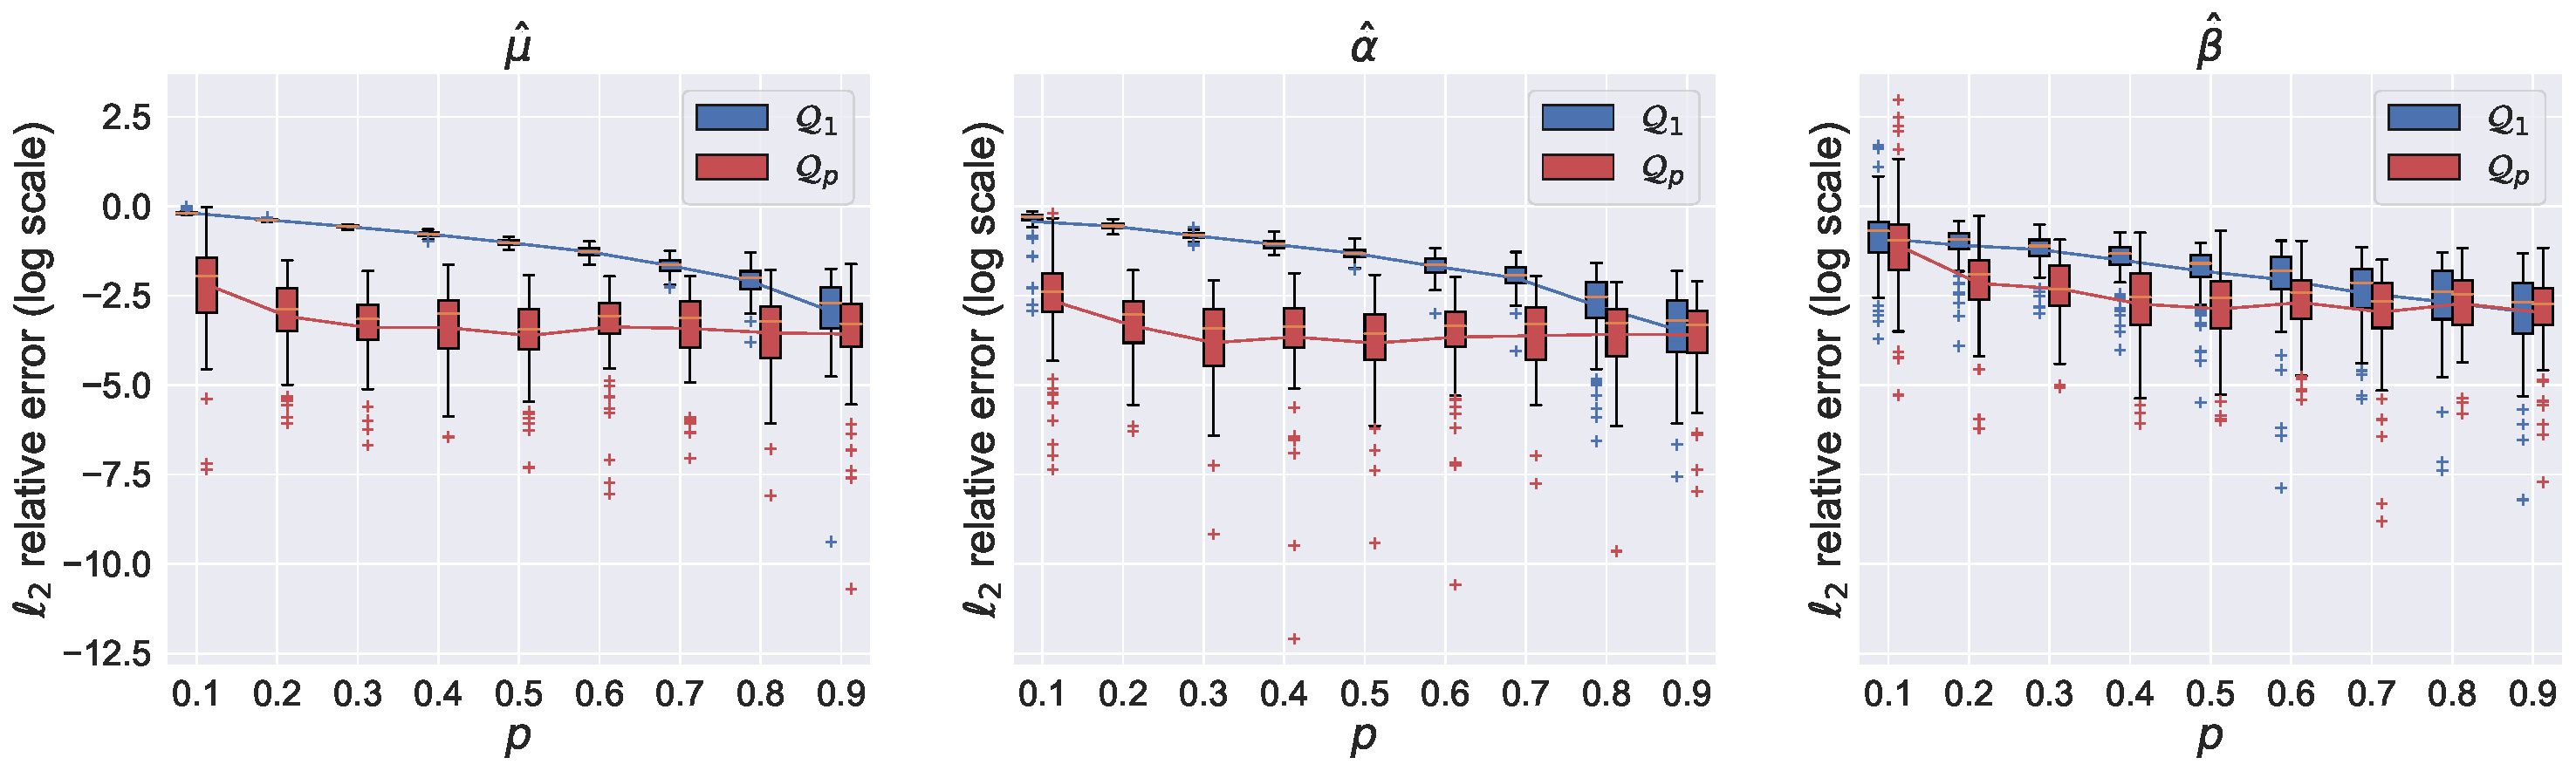
\includegraphics[width=1.0\textwidth]{images/chapter5/l2_error_same_information.pdf} 
        \caption{
        }
        \label{fig:chap5_l2_error_same_information}
      \end{figure}




\begin{subappendices}
    \section{Proof of Proposition~\ref{prop:chap5_spectral_thinning}}\label{appendix:chap5_proof_spectral_thinning}
        Let $H_p$ be a $p$-thinning of a stationary point process $H$ admitting a spectral density function $f$.
        The stationarity of $H_p$ is given by the fact that the variables $(Z_k)_{k\in\ZZ}$ are i.i.d. and so for any integer $r$, 
        for any $B_1\ldots, B_r \in\mathcal{B}^c$, 
        the random vector $(N_p(B_k)_{k=1:r})$ has the same distribution as $(N_p(B_k+t)_{k=1:r})$,
        for any $t\in\RR$.
        We will then denote $\Gamma_p$ and $f_p$ respectively the Bartlett spectrum and spectral density function of $H_p$

        In order to establish Equation~\eqref{eq:chap5_spectral_thinning}, we will leverage Theorem~\ref{th:chap5_spectral_marked}.
        We consider then the marked version $\bar H$ of $H$ where the marks $Z_k$ are i.i.d. Bernoulli distributions with common probability $p$.

        Let $\varphi, \psi \in \mathcal{S}$, we define, for all $x,z\in\RR\times\{0,1\}$, the functions:
        \[\varphi^\star(x,z) = \varphi(x)z\,,\qquad \psi^\star(x,z) = \psi(x)z\,.\]

        Let us verify that these functions verify the conditions of Theorem~\ref{th:chap5_spectral_marked}. 
        Without lose of generality, we will work uniquely with $\varphi^\star$, as the arguments are exactly the same for $\psi^\star$.
        
        For any $x\in\RR$, $\varphi^\star(x, Z) = \varphi(x)Z$ for Z a Bernoulli distribution of parameter $p$.
        It follows that $\varphi^\star(x, Z)$ admits a first and second order moment, and as $\varphi\in\mathcal{S}$, 
        $\varphi(x)Z$ is integrable and twice integrable, which shows that:
                \[
                \int_{\RR}{\EE\left[|\varphi^\star(x, Z)|\right]\dd(x)} < +\infty\,,\qquad 
                \int_{\RR}{\EE\left[\varphi^\star(x, Z)^2\right]\dd(x)} < +\infty\,.
                \]
        Furthermore, for any $x\in\RR$, $\bar \varphi(x) = \varphi(x)\EE[Z] = p \varphi(x)$,
        and so, as the Schwartz space is closed under scalar mutliplication, it follows that $\bar \varphi\in\mathcal{S}$.

        We can then apply Equation~\eqref{eq:chap5_marked_spectrum} to our marked process $\bar H$. 
        For this, let us notice that:
        \[
            \sum_{k\in\ZZ}{\varphi^\star(T_k, Z_k)} = \sum_{k\in\ZZ}{\varphi(T_k)Z_k} = \int_{\RR}{\varphi(t) H_p(\dd t)}\,,
        \]
        with the same expression holding for $\psi^\star$ and $\psi$. 
        So, the left-hand side of Equation~\eqref{eq:chap5_marked_spectrum} reads:
        \begin{align}
            \Cov\left(\sum_{k\in\ZZ}{\varphi^\star(T_k, Z_k)}, \sum_{k\in\ZZ}{\psi^\star(T_k, Z_k)}\right) &=
            \Cov\left(\int_{\RR}{\varphi(t) H_p(\dd t)}, \int_{\RR}{\psi(t) H_p(\dd t)}\right) \nonumber\\
            &= \int_{\RR}{\tilde \varphi(\omega)\tilde \psi(-\omega)\,\Gamma_p(\dd\omega)}\,,\label{eq:chap5_leftside_proof_thinning}
        \end{align}
        where the last equality comes from Equation~\eqref{eq:chap5_bartlett_covariance}.

        For the left-hand side, let us remark that $\bar \varphi(x) = p \varphi(x)$ for any $x\in\RR$ and so, for any $\omega\in\RR$,
        \[
            \tilde {\bar \varphi}(\omega) = p \tilde \varphi(\omega)\,,
        \]
        and,
        \[\tilde \phi^\star(\omega, Z) = \tilde \phi(\omega)Z\,.\]

        The right-hand side of Equation~\eqref{eq:chap5_marked_spectrum} becomes:

        \begin{align}
            \int_{\RR}{\tilde {\bar\varphi} (\omega) \tilde{\bar \psi} (-\omega)\,\Gamma(\dd \omega)} 
        + &\int_{\RR}{\Cov\left( \tilde \varphi^\star(\omega, Z), \tilde \psi^\star (-\omega, Z)\,M_1(\dd \omega)\right)} \nonumber\\
        &= \int_{\RR}{p^2 \tilde {\varphi} (\omega) \tilde{\psi} (-\omega)\,\Gamma(\dd \omega)} 
        + \int_{\RR}{\tilde \varphi(\omega)\tilde \psi(\omega) \Cov\left(Z,Z\right)M_1(\dd \omega)} \nonumber\\
        &= \int_{\RR}{\tilde {\varphi} (\omega) \tilde{\psi} (-\omega)\,(p^2\Gamma(\dd \omega) + p(1-p) M_1(\dd \omega))}\,.\label{eq:chap5_rightside_proof_thinning}
        \end{align}

        By combining both sides (Equations~\eqref{eq:chap5_leftside_proof_thinning} and \eqref{eq:chap5_rightside_proof_thinning}) it follows that,
        for any $\varphi, \psi\in\mathcal{S}$:
        \[
            \int_{\RR}{\tilde \varphi(\omega)\tilde \psi(-\omega)\,\Gamma_p(\dd\omega)} = \int_{\RR}{\tilde {\varphi} (\omega) \tilde{\psi} (-\omega)\,(p^2\Gamma(\dd \omega) + p(1-p) M_1(\dd \omega))}\,.
        \]
        
        As this equality holds for any functions in the Schwartz space \textbf{Add reference}, then,
        \[\Gamma_p = p^2 \Gamma + p(1-p) M_1\,,\]
        and as $M_1 = m_1 \ell_{\RR}$,
        \[f_p(\omega) = p^2 f(\omega) + p(1-p) m_1\,,\]
        which achieves the proof.





    \section{Proof of Proposition~\ref{prop:chap5_identifiability_thinning}}\label{appendix:chap5_proof_identifiability_thinning}

    Let $\theta = (\mu, \alpha, \beta, p)$ and $\theta' = (\mu', \alpha', \beta', p')$ be two admissible parameter for model $\mathcal{Q}$.

    In order to prove that model $\mathcal{Q}$ is identifiable if and only if one of four parameters is fixed, 
    we will begin by retrieving the system of Equations~\eqref{eq:chap5_nonidentifiable_parameters}
    and verify that it defines an admissible parameter for $\mathcal{Q}$.
    Subsequently we will verify that by fixing one parameter, we retrieve the identifiability of the model.
    
    We begin by assuming that $f_\theta = f_{\theta'}$.
    By Equation~\eqref{eq:chap5_spectral_exponential}, this equality reads:
    \[\forall \omega \in \RR,\quad 
    \frac{\mu p }{1-\alpha}\left(1 + p \frac{\beta^2 \alpha (2-\alpha)}{\beta^2(1-\alpha)^2 + 4 \pi^2 \omega^2}\right) = 
    \frac{\mu' p' }{1-\alpha'}\left(1 + p' \frac{{\beta'}^2 \alpha' (2-\alpha')}{{\beta'}^2(1-\alpha')^2 + 4 \pi^2 \omega^2}\right)\,.
    \]

    Let us remark that a sufficient condition for both sides to be equal, 
    for all $\omega \in \RR$,
    is that the following system of equations is verified:

    \begin{equation}\label{eq:chap5_system_identifiability}
        \begin{cases}
            \frac{\mu p }{1-\alpha} = \frac{\mu' p'}{1-\alpha'}\\
            p \beta^2 \alpha(2-\alpha) = p' {\beta'}^2 \alpha'(2-\alpha')\\
            \beta (1-\alpha) = \beta' (1-\alpha')\,,
        \end{cases}
    \end{equation}
    as this would mean that the three constants (w.r.t. $\omega$) in both sides are equal.
    In fact this is also a necessary condition as the three equalities can be retrieved for $f(0)$, $\lim_{\omega\to+\infty}{f(\omega)}$ and $f(1)$
    and combining the equations.

    Let $\kappa\in(0, 1/p)$ and $p' = \kappa p$, which reduces the system of Equations~\eqref{eq:chap5_system_identifiability} to:

    \begin{subnumcases}{}
            \frac{\mu}{1-\alpha} = \frac{\mu' \kappa}{1-\alpha'}\label{eq:chap5_system_identifiability1}\\
            \beta^2 \alpha(2-\alpha) = \kappa {\beta'}^2 \alpha'(2-\alpha')\label{eq:chap5_system_identifiability2}\\
            \beta (1-\alpha) = \beta' (1-\alpha')\,,\label{eq:chap5_system_identifiability3}
    \end{subnumcases}

    As $\alpha > 1$, $\alpha'>1$, $\beta>0$ and $\beta'>0$, 
    Equation~\eqref{eq:chap5_system_identifiability3} can be expressed as:
    \[{\beta'}^2 = \frac{\beta^2(1-\alpha)^2}{(1-\alpha')^2}\,,\]
    and by replacing ${\beta'}^2$ in Equation~\eqref{eq:chap5_system_identifiability2}, we obtain:
    \begin{align}
        &\frac{\alpha (2-\alpha)}{(1-\alpha)^2} = \kappa \frac{\alpha' (2-\alpha')}{(1-\alpha')^2}\label{eq:chap5_alpha_equality} \\
        \iff\quad & \frac{1 - (1-\alpha)^2}{(1-\alpha)^2} = \kappa \frac{1 - (1-\alpha')^2}{(1-\alpha')^2}\nonumber \\
        \iff\quad & 1 + \frac{1}{\kappa}\left(\frac{1}{(1-\alpha)^2} - 1\right) = \frac{1}{(1-\alpha')^2}\nonumber\,,
    \end{align}
    and as $\alpha \in(0,1)$, the left-side term is positive and so:
    \[\alpha' = 1 - \frac{1}{\sqrt{1 + \frac{1}{\kappa}\left(\frac{1}{(1-\alpha)^2} - 1\right)}}\,.\]

    We can then obtain the explicit expressions of $\mu'$ and $\beta'$ with Equations~\eqref{eq:chap5_system_identifiability1} and \eqref{eq:chap5_system_identifiability3}
    providing the following system:
    
    \begin{equation}\label{eq:chap5_system_parameters}
        \begin{cases*}
            \mu' = \frac{\mu(1-\alpha')}{\kappa(1-\alpha)}\\
            \alpha' = 1 - \frac{1}{\sqrt{1 + \frac{1}{\kappa}\left(\frac{1}{(1-\alpha)^2} - 1\right)}}\\
            \beta' = \beta \frac{1-\alpha}{1-\alpha'}\\
            p' = \kappa p
        \end{cases*}
        \quad\iff\quad
        \begin{cases}
            \mu' = \frac{\mu}{\kappa(1-\alpha)\sqrt{1 + \frac{1}{\kappa}\left(\frac{1}{(1-\alpha)^2} - 1\right)}}\\
            \alpha' = 1 - \frac{1}{\sqrt{1 + \frac{1}{\kappa}\left(\frac{1}{(1-\alpha)^2} - 1\right)}}\\
            \beta' = \beta (1-\alpha) \sqrt{1 + \frac{1}{\kappa}\left(\frac{1}{(1-\alpha)^2} - 1\right)}\\
            p' = \kappa p\,.
        \end{cases}
    \end{equation}
    
    To verify that, for any $\kappa\in(0,1/p)$, parameter $\theta' = (\mu', \alpha', \beta', p')$ is an admissible parameter,
    we have to make sure that $\theta' \in \Theta = \RR_{>0}\times (0,1) \times \RR_{>0} \times (0,1)$.
    Let $\theta = (\mu, \alpha, \beta, p)\in\Theta$, $\kappa\in(0,1/p)$ and $\theta'$ defined by Equations~\eqref{eq:chap5_system_parameters}.
    For such a $\kappa$, $p'\in(0,1)$ is immediately verified.

    The rest of the conditions are verified if and only if: 
    \[\sqrt{1 + \frac{1}{\kappa}\left(\frac{1}{(1-\alpha)^2} - 1\right)} > 1 \iff \frac{1}{(1-\alpha)^2} - 1 > 0\\,.\]
    This is immediate as $\alpha\in(0,1)$ and so $\theta'\in\Theta$. 
    From Equations~\eqref{eq:chap5_system_parameters}
    we can see that $\theta'=\theta$ and we've proven that $f_\theta = f_{\theta'}$,
    so model $\mathcal{Q}$ is not identifiable.

    Lastly, let us show that if any of the four parameters is known then the model defined by the remaining triplet is identidiable.
    By considering the previously established equations (see Equations~\eqref{eq:chap5_alpha_equality} and \eqref{eq:chap5_system_parameters}), 
    we know that for $\theta = (\mu, \alpha, \beta, p)\in\Theta$ and $\theta' = (\mu', \alpha', \beta', p')\in\Theta$:
    \begin{equation}\label{eq:chap5_system_fixed}
        f_{\theta} = f_{\theta'} \quad\iff\quad 
        \begin{cases*}
            \mu' = \frac{\mu(1-\alpha')}{\kappa(1-\alpha)}\\
            \frac{\alpha (2-\alpha)}{(1-\alpha)^2} = \kappa \frac{\alpha' (2-\alpha')}{(1-\alpha')^2}\\     
            \beta' = \beta \frac{1-\alpha}{1-\alpha'}\\
            p' = \kappa p
        \end{cases*}\,.
    \end{equation}
    \begin{itemize}
        \item If $\mu = \mu'$, the system of Equations~\eqref{eq:chap5_system_fixed} reduces to:
        \begin{equation*}
            \begin{cases*}
                \kappa = \frac{(1-\alpha')}{(1-\alpha)}\\
                \kappa \frac{\alpha' (2-\alpha')}{(1-\alpha')^2} = \frac{\alpha (2-\alpha)}{(1-\alpha)^2}\\     
                \beta' = \frac{\beta}{\kappa}\\
                p' = \kappa p
            \end{cases*}\quad\iff\quad
            \begin{cases*}
                \kappa = \frac{(1-\alpha')}{(1-\alpha)}\\
                \frac{\alpha' (2-\alpha')}{(1-\alpha')} = \frac{\alpha (2-\alpha)}{(1-\alpha)}\\     
                \beta' = \frac{\beta}{\kappa}\\
                p' = \kappa p
            \end{cases*}\,.
        \end{equation*}

        As $\alpha\in(0,1)$ and $\alpha'\in(0,1)$, the second equation implies that $\alpha=\alpha'$ and so $\kappa=1$ and $\beta'=\beta$.

        \item If $\alpha = \alpha'$, the second equation in \eqref{eq:chap5_system_fixed} implies directly that $\kappa=1$ and so all other equalities follow.
        \item If $\beta = \beta'$, the third equation in \eqref{eq:chap5_system_fixed} implies that $\alpha=\alpha'$ and by the previous point all other equalities hold.
        \item If $p = p'$, $\kappa=1$ and the rest of equalities are verified.
        
        This shows that whenever one of the parameters is fixed, $f_\theta = f_{\theta'}$ implies $\theta = \theta'$. This achieves the proof.

    \end{itemize}



\end{subappendices}